\documentclass[12pt]{article}

\title{University of Massachusetts Lowell \\ [3cm]
{\vspace{-2cm}\rule{\linewidth}{0.5mm}
Some Application of Singular Value Decomposition\\
\rule{\linewidth}{0.5mm}\vspace{-0.5cm}}\\[3cm]}

\author{{Author: Jessica C. Barhouane}\\
{Faculty Advisor: Hung Phan}\\[7cm]
{Department of Mathematical Sciences}}

\date{May 2, 2023}

\usepackage{indentfirst}
\usepackage{amsmath}
\usepackage{amsfonts}
\usepackage{amssymb}
\usepackage{graphicx}
 \usepackage{sidecap}
 \usepackage[table]{xcolor}
 \usepackage[fullpage]{geometry}
 \usepackage{nicematrix}
 \usepackage{listings}

\definecolor{codegreen}{rgb}{0,0.6,0}
\definecolor{codegray}{rgb}{0.5,0.5,0.5}
\definecolor{codepurple}{rgb}{0.58,0,0.82}
\definecolor{backcolour}{rgb}{0.95,0.95,0.92}

\lstdefinestyle{mystyle}{
    backgroundcolor=\color{backcolour},   
    commentstyle=\color{codegreen},
    keywordstyle=\color{magenta},
    numberstyle=\tiny\color{codegray},
    stringstyle=\color{codepurple},
    basicstyle=\ttfamily\footnotesize,
    breakatwhitespace=false,         
    breaklines=true,                 
    captionpos=b,                    
    keepspaces=true,                 
    numbers=left,                    
    numbersep=5pt,                  
    showspaces=false,                
    showstringspaces=false,
    showtabs=false,                  
    tabsize=2
}

\lstset{style=mystyle}

\lstdefinestyle{input}{
  language=,
  basicstyle=\ttfamily\color{white},
  backgroundcolor=\color{black},
  numbers=none,
  frame=none,
  columns=fullflexible,
  showstringspaces=false,
  upquote=true,
  moredelim=[is][\bfseries\color{green!50!black}]{<}{>},
  moredelim=[is][\color{white}]{\$\$}{\$\$}
}
 
\begin{document}

\maketitle
\newpage

\begin{center} 
    \LARGE\textbf{Abstract\\}
\end{center}

The Singular Value Decomposition (SVD) is a powerful and adaptable linear algebra algorithm that has gained significant importance in numerous fields today. This paper delves into a thorough exploration of the various algorithms and industries that harness SVD for successful implementation in data compression, modification, and detection.

To begin, we will provide an in-depth examination of the fundamental matrix operations of SVD, clarifying the steps involved in its computation. We will offer a detailed overview of how SVD operates, as well as discuss other related SVD-based algorithms, such as Principal Component Analysis (PCA) and Collaborative Filtering (CF).  PCA, for instance, is an algorithm that leverages SVD to transform the original data into a set of linearly uncorrelated variables called principal components, while CF is a technique commonly used in recommender systems that employs SVD to discover latent factors.

Following this, we will investigate several industries that utilize SVD, exploring the diverse applications of SVD-based algorithms in areas such as image processing, facial recognition, and recommender systems. This investigation will provide a solid understanding of how SVD can effectively compress and identify unique patterns and features in large, complex datasets.

Ultimately, this paper strives to demonstrate the versatility and practicality of SVD in the modern technology sector. By reviewing its numerous applications across various machine learning topics, we will emphasize the vital importance of SVD in today's rapidly evolving technological world. This thorough analysis serves to further our understanding of SVD's potential and reinforces its status as an essential tool in the realm of data processing and machine learning.
\newpage
\tableofcontents
\newpage
\section{Introduction}
\par Singular Value Decomposition (SVD) is a well-known linear algebra algorithm that has led to numerous breakthroughs in a variety of fields, including machine learning, data analysis, and computer science. This paper strives to provide an in-depth overview of Singular Value Decomposition (SVD) and its various applications, particularly in the technology sector. By exploring the historical development of SVD, explaining its mathematical principles, and examining modern utilization of SVD, this paper emphasizes the importance and versatility of SVD as a powerful linear algebra algorithm.

SVD is the process of decomposing a matrix to obtain its singular values. This decomposition allows for the retrieval or compression of data from large datasets with efficiency and precision by eliminating unnecessary or redundant data. In this paper, we will review the history of SVD, the properties and process of decomposing a matrix to obtain the singular values, and demonstrate how SVD is implemented in a variety ways.

SVD was initially discovered by Italian mathematician Eugenio Beltrami in 1873, and French mathematician Camille Jordan in 1874. Both mathematicians independently worked on it and are considered the founders of SVD. Beltrami, the first to publish, had his work appear in the Journal of Mathematics for Italian Students. Later contributors to SVD included James Joseph Sylvester, Erhard Schmidt, and Hermann Weyl.

SVD has undergone many transformations over the years. Although discovered in the 19th century, it was not until the 1970s, due to advancements in computers and technology, that SVD became a widely used algorithm. Since then, it has been implemented in various industries requiring advanced computation. As technology continues to progress, the use of the SVD algorithm is expected to grow. Today, numerous companies, programming languages, and other algorithms utilize SVD to enhance performance. Some of the larger companies, such as Google, Netflix, and Facebook, use SVD or SVD-based algorithms for their recommendation systems. These systems recommend content, products, or advertisements to customers to increase engagement. Programming languages, including Python, MATLAB, C++, Julia, and others, have been structured or modified to decompose matrices and find singular values, enabling the development of processes and applications that have become essential to our society today. The widespread adoption and continuous development of SVD-based techniques underscore their importance in solving complex problems and discovering patterns within massive datasets.

The goal of this paper is to provide a deep understanding of SVD's foundational concepts, applications, and importance in modern technology, offering insights into its potential future developments and contributions to various fields.

\section{Preliminaries}
In this section, we will review essential linear algebra concepts and operations that serve as the foundation for understanding the Singular Value Decomposition (SVD) algorithm, as well as the steps required to compute SVD. We will cover matrix multiplication, eigenvalues and eigenvectors, singular value decomposition, and low-rank approximation. By revisiting these fundamental concepts, we aim to establish a solid foundation that allows for a deeper understanding and further exploration of SVD and its practical applications.

\subsection{Linear Algebra Basics}
Singular Value Decomposition (SVD) is a mathematical algorithm used in linear algebra that involves several matrix operations to access important aspects of data. In order to understand how to compute SVD, it's crucial to review and grasp basic matrix operations in linear algebra. These operations include matrix multiplication and computing the eigenvalues and eigenvectors of a square matrix. By reviewing some of these operations, we can gain a better understanding of how to compute the SVD algorithm. Before proceeding to the computation of SVD, it's essential to first establish a solid understanding of these fundamental matrix operations.

\subsubsection{Matrix multiplication}
In this section, we will begin by reviewing matrix multiplication. When multiplying matrices together, it's important to note that matrix multiplication is not commutative, meaning $A \times B \neq B \times A$. To multiply two matrices together, the number of rows in the first matrix must be equal to the number of columns in the second matrix, and vice versa. Another important property of multiplying matrices is that if we have $A$ as an $m \times n$ matrix and $B$ as an $n \times m$ matrix, then $AB$ is an $m \times m$ matrix and $BA$ is an $n \times n$ matrix. When calculating each element in the product of two matrices, one should multiply each element in the first row of the first matrix by the corresponding element in the first column of the second matrix, and then compute the sum of the acquired products. When an element in the resulting matrix is computed using row 'M' of the first matrix and column 'N' of the second matrix, the element is placed in the corresponding position (M, N) within the resulting matrix.

The example below demonstrates how we multiply two matrices together.

Let $C = A \times B$ and let $D = B \times A$.

\begin{center}
$A = $
\begin{bmatrix}
3 & 0 & 2 \cr
0 & 4 & 2 \cr\end{bmatrix}
and $B = $
\begin{bmatrix}
1 & 0\cr
3 & 2\cr
3 & 4\cr
\end{bmatrix}\
\end{center}
Since $A$ is a $2 \times 3$ matrix and $B$ is a $3 \times 2$ matrix, $C$ will be a $2 \times 2$ matrix and $D$ will be a $3 \times 3$ matrix. Computing each element, we get,

So the resultant matrices are,
\begin{center}
$C = $
\begin{bmatrix}
9 & 8 \cr
18 & 6 \cr
\end{bmatrix}
and $D = $
\begin{bmatrix}
3 & 0 & 2 \cr
9 & 8 & 10 \cr
9 & 16 & 14 \cr
\end{bmatrix}
\end{center}
\subsubsection{Eigenvalues and eigenvectors}
Eigenvalues and eigenvectors are both essential concepts in linear algebra and form the backbone of SVD. They play an important role in various processes and are used in numerous industries today. In this section, we will review the computation of eigenvalues and eigenvectors and provide an overview of industries that make use of them. In the next section, when we compute Singular Value Decomposition, we will demonstrate how they are utilized in the SVD algorithm.\\
\newline
\noindent \textbf{Definition} Let $A$ be an $n \times n$ matrix.
An eigenvector of A is a nonzero vector $v$ in $R^n$ such that $Av$ = $\lambda v$ for some scalar $\lambda$.\\
\newline
\textbf{Definition} An eigenvalue of $A$ is a scalar $\lambda$ such that the equation $Av$ = $\lambda v$ has a nontrivial solution.\\

If $Av = \lambda v$ for $v \neq 0$, we say that $\lambda$ is the eigenvalue for $v$, and that $v$ is an eigenvector for $\lambda$.
\begin{center}
\tiny 
Definitions from https://textbooks.math.gatech.edu/ila/eigenvectors.html    
\end{center}
\newpage
\begin{center}
\textbf{Eigenvalues}    
\end{center}\\

Eigenvalues play an important role in a diverse range of fields, such as physics, engineering, and computer graphics. They facilitate our understanding of linear transformations and matrices by revealing how a matrix can shrink or expand a vector in any direction. Consequently, eigenvalues enable us to comprehend complex systems and tackle various computational problems more effectively.\\

To find the eigenvalues of a given $n \times n$ matrix $A$, we must first derive the characteristic equation. This process involves calculating the difference between $A$ and $\lambda I$, where $I$ represents the identity matrix. After determining the resultant matrix, we compute its determinant. Finally, we find the roots of the characteristic equation, which correspond to the eigenvalues.\\

 Here is an example of calculating the eigenvalues of a $3 \times 3$ matrix:
 \newline
 \begin{center}
 $A = $
     \begin{bmatrix}
         3 & 6 & 1 \cr
         2 & 4 & 5 \cr
         6 & 0 & 2 \cr
     \end{bmatrix}
 \end{center} \\
 \newline 
 \par First we must subtract $\lambda I$ from the matrix $A$. Doing so we get, \\
 \begin{center}
 $A - \lambda I = $
     \begin{bmatrix}
         2 & 3 & 4 \cr
         4 & 3 & 2 \cr
         2 & 2 & 2 \cr
     \end{bmatrix}
     - 
     \begin{bmatrix}
         \lambda & 0 & 0 \cr
         0 & \lambda & 0 \cr
         0 & 0 & \lambda \cr
     \end{bmatrix}
     =
     \begin{bmatrix}
         2 - \lambda & 3 & 4 \cr
         4 & 3 - \lambda & 2 \cr
         2 & 2 & 2 - \lambda \cr
     \end{bmatrix}     
 \end{center}\\
\newline
\par Next, we determine the characteristic equation by calculating the determinant of the matrix. For square matrices larger than $2 \times 2$, we utilize cofactor expansion to obtain the characteristic equation. Cofactor expansion involves selecting an element, removing its corresponding row and column, and computing the sum of the products along the remaining diagonals. The cofactor expansion for our $3 \times 3$ matrix is demonstrated as follows: \\
 
\begin{center}
$A = $
    \begin{bmatrix}
         2 - \lambda & 3 & 4 \cr
         4 & 3 - \lambda & 2 \cr
         2 & 2 & 2 - \lambda \cr
    \end{bmatrix}
\end{center}\\

\par The resulting characteristic equation is as follows: \\

\newline
$(2 - \lambda )((3 - \lambda )(2 - \lambda) - 2 \times 2) - 3(4(2 - \lambda) - 2 \times 2) + 4(4 \times 2 - (3 - \lambda) \times 2) = 0$\\
\newline
\par Upon simplifying the equation, we obtain:
\newline
\begin{center}
$-\lambda ^3 + 7 \lambda ^2 + 8 \lambda = 0$ \\
\end{center}
\newline
\par Factoring the equation, we find:
\newline
\begin{center}
$-\lambda (\lambda - 8)(\lambda + 1)$\\
\end{center}
\newline
\par This results in the following eigenvalues:
\newline
\begin{center}
$\lambda _1 = 8, \lambda _2 = 0, \lambda _3 = -1$\\
\end{center}
\newline

 \begin{center}
\textbf{Eigenvectors}    
\end{center}\par 
Eigenvectors are a vital concept in linear algebra, as they highlight the key features of a matrix. By determining a matrix's eigenvectors, we can better understand how it transforms or preserves specific directions in space. This knowledge is particularly useful in fields such as image processing, pattern recognition, and data analysis, where identifying the most important elements of the data is essential.\

\par To discover an eigenvector, we first use one of the eigenvalues obtained in previous steps in the equation $A - \lambda I$. We then multiply the resulting matrix by a vector that includes $x_1,..., x_n$ and set it equal to 0. Afterward, we rewrite the matrix in reduced row echelon form and solve for x. This procedure is carried out for each eigenvalue.\\
\newline
\noindent \textbf{Step 1:} Set up the characteristic equation to find the eigenvalues by subtracting \hspace*{1.4cm} $\lambda$ from the diagonal elements of the matrix and solving the resulting\\ \hspace*{1.4cm} determinant equal to zero.
\begin{center}
    \begin{bmatrix}
         2 - \lambda & 3 & 4 \cr
         4 & 3 - \lambda & 2 \cr
         2 & 2 & 2 - \lambda \cr
     \end{bmatrix}     
     \begin{bmatrix}
         x_1\cr
         x_2\cr
         x_3\cr
     \end{bmatrix}
     =
     \begin{bmatrix}
         0\cr
         0\cr
         0\cr
     \end{bmatrix}
\end{center}
\newpage
\noindent \textbf{Step 2:} Choosing $\lambda _1$ we obtain,
\begin{center}
    \begin{bmatrix}
         2 - 8 & 3 & 4 \cr
         4 & 3 - 8 & 2 \cr
         2 & 2 & 2 - 8 \cr
     \end{bmatrix}    
     = 
     \begin{bmatrix}
         -6 & 3 & 4 \cr
         4 & -5 & 2 \cr
         2 & 2 & -6 \cr
     \end{bmatrix}
\end{center}
\textbf{Step 3:} Transform the matrix to reduced row echelon form.
\begin{center}
    
    \begin{bmatrix}
        -6 & 3 & 4 \cr
        4 & -5 & 2 \cr
        2 & 2 & -6 \cr
    \end{bmatrix}
    \rightarrow
    \begin{bmatrix}
        1 & 0 & \frac{-13}{9}\cr
        0 & 1 & \frac{-14}{9}\cr
        0 & 0 & 0 \cr
    \end{bmatrix}\\
\end{center}
\textbf{Step 4:} Utilizing the reduced row echelon form, we can determine the eigenvectors:\\
\begin{center}
    \begin{bmatrix}
        1 & 0 & - \frac{13}{9}\cr
        0 & 1 & - \frac{14}{9}\cr
        0 & 0 & 0 \cr
    \end{bmatrix}
     \begin{bmatrix}
         x_1\cr
         x_2\cr
         x_3\cr
     \end{bmatrix}
     =
     \begin{bmatrix}
         0\cr
         0\cr
         0\cr
     \end{bmatrix}\\
\end{center}
\par With the matrix now in reduced form, we can calculate our first eigenvector. We extract each equation from the matrix, set them equal to zero, and then solve.\\
\begin{center}
    1. $x_1 - \frac{13}{9} x_3 = 0  \rightarrow  x_1 = \frac{13}{9} x_3$\\
    \vspace{.5cm}
    2. $x_2 - \frac{14}{9} x_3 = 0  \rightarrow  x_2 = \frac{14}{9} x_3$\\
\end{center}

\newline
Letting $x_3 = 1$ yields the vector, \\

\begin{center}
     $v_1 = $
     \begin{bmatrix}
         \frac{13}{9}\cr
         \frac{14}{9}\cr
         1\cr
     \end{bmatrix}
\end{center}

With the first eigenvector found, we can now proceed to find the remaining eigenvectors by repeating the process for the remaining eigenvalues. After obtaining all the eigenvectors, we can analyze the matrix's behavior and its effect on space, which can be beneficial for various applications, such as image processing, pattern recognition, and data analysis.
     
\subsection{Singular Value Decomposition}

\noindent \textbf{Definition 4.7.2}
The singular value decomposition (SVD) of an $m x n$ real or complex matrix $M$ is a factorization of the form
\begin{center}
$M = U \Sigma V^T$
\end{center}
where $U$ is an $m x n$ real or complex unitary matrix, $\Sigma$ = diag($\sigma_1\ge...\ge\sigma_k\ge0$) where 
$\sigma_1\ge...\ge\sigma_k\ge0$ $k$ = min($m, n$), is an $m x n$ rectangular diagonal matrix with non-negative real numbers on the diagonal, and $V$ is an $n x n$ real or complex unitary matrix. The diagonal entries $\sigma_i$ of $\Sigma$ are known as the singular values of $M$. The columns of $U$ and the columns of $V$ are called the left-singular and right-singular vectors of $M$.
\begin{center}
\tiny
Definition from Linear Algebra by Shen, L., Wang, Haohao, and Wijdylo, J. 2019
\end{center}
\subsubsection{Computation}
Computing the SVD of a matrix involves several steps, as mentioned. Here's a step-by-step breakdown of the process to compute $U \Sigma V^T$ for a given matrix $A$:
\begin{enumerate}
    \item Calculate the product of $A$ and its transpose, $A^T$: Compute $AA^T$ and $A^TA$. These products will be used to find the eigenvalues and eigenvectors for matrices $U$ and $V$.

    \item Compute the eigenvalues of $AA^T$ and $A^TA$. The eigenvalues of $AA^T$ will be used to find the singular values in matrix $\Sigma$ and the eigenvectors for matrix $V$ and the eigenvalues of $AA^T$ will be used to the find the eigenvectors for matrix $U$.

    \item Calculate the singular values for matrix $\Sigma$: Take the square root of the eigenvalues obtained from $AA^T$ (or $A^TA$ as they should have the same non-zero eigenvalues) and arrange them in decreasing order along the diagonal of matrix $\Sigma$.

    \item Find the eigenvectors of $AA^T$ to form matrix $U$: Use the eigenvalues computed in step 2 to find the corresponding eigenvectors of $AA^T$. These eigenvectors will form the columns of matrix $U$.

    \item Find the eigenvectors of $A^TA$ to form matrix $V$: Use the eigenvalues computed in step 2 to find the corresponding eigenvectors of $A^TA$. These eigenvectors will form the columns of matrix $V$. Then, compute the transpose of matrix $V$, denoted as $V^T$.

    \item Assemble the SVD: Combine the computed matrices $U$, $\Sigma$, and $V^T$ to form the SVD of matrix $A$. The final expression should be:
    \begin{center}
    $A = U \Sigma V^T$
    \end{center}
\end{enumerate}
By following these steps, we can compute the SVD of any given matrix, revealing insights about its structure and properties. SVD is widely used in various fields, including data analysis, signal processing, and dimensionality reduction.\\
\newline
Example of SVD on matrix $A$,
\begin{center}
Let $A=\begin{bmatrix}
1 &  2  & 1 \cr
2 & -1 & 2 \cr
\end{bmatrix}$. \\
\end{center}
\textbf{Step 1:} Compute $AA^T$ and $A^TA$\\
\newline

\hspace{2.5cm} $AA^T$ = 
$\begin{bmatrix}
1 &  2  & 1 \cr
2 & -1 & 2 \cr
\end{bmatrix}$
$\begin{bmatrix}
1 &  2 \cr
2 & -1 \cr
1 & 2 \cr
\end{bmatrix}$ 
=
$\begin{bmatrix}
6 & 2 \cr
2 & 9 \cr
\end{bmatrix}$\\
\newline

\hspace{2.5cm} $A^TA =$
\begin{bmatrix}
1 &  2  & 1 \cr
2 & -1 & 2 \cr
\end{bmatrix}
\begin{bmatrix}
1 &  2 \cr
2 & -1 \cr
1 & 2 \cr
\end{bmatrix}
=
\begin{bmatrix}
    5 & 0 & 5 \cr
    0 & 5 & 0 \cr
    5 & 0 & 5 \cr
\end{bmatrix}
\\
\newline

\noindent \textbf{Step 2:} Obtain the characteristic equations\\
\newline

\hspace{2.5cm} $AA^T - \lambda I$ = 
$\begin{bmatrix}
6 - \lambda & 2 \cr
2 & 9 - \lambda \cr
\end{bmatrix}$\\
\newline

\hspace{2.5cm}$A^TA - \lambda I$ =
\begin{bmatrix}
    5 - \lambda & 0 & 5 \cr
    0 & 5 - \lambda & 0 \cr
    5 & 0 & 5 - \lambda \cr
\end{bmatrix}

\begin{center}
    \begin{tabular}{|c|c|}
        \hline   
        \textbf{$AA^T$} &  \textbf{$A^TA$}\\
        0 = \lambda^2 - 15\lambda+50  & -\lambda ^3 + 15 \lambda ^2 - 50 \lambda\\
        \lambda_1 = 10, \lambda_2 = 5 & \lambda_1 = 0, \lambda_2 = 5, \lambda_3 = 10\\ 
        \hline
    \end{tabular}
\end{center}
\textbf{Step 3:} Compute the Eigenvectors of $AA^T$ for $U$ and $A^TA$ for $V$
\begin{center}
$u_1 =$
    \begin{bmatrix}
      \frac{2 \sqrt{2}}{5}\cr
      \frac{2 \sqrt{2}}{5}\cr
    \end{bmatrix}
    $u_2 =$
    \begin{bmatrix}
      \frac{2 \sqrt{2}}{5}\cr
      \frac{2 \sqrt{2}}{5}\cr
    \end{bmatrix}
 $v_1 = $ 
$\begin{bmatrix}
-\frac{\sqrt{2}}{2} \cr
0 \cr
\frac{\sqrt{2}}{2} \cr
\end{bmatrix}$
$v_2 = $ 
$\begin{bmatrix}
0 \cr
1 \cr
0 \cr
\end{bmatrix}$
$v_3 = $ 
$\begin{bmatrix}
\frac{\sqrt{2}}{2} \cr
0 \cr
\frac{\sqrt{2}}{2} \cr
\end{bmatrix}$
\end{center}
\textbf{Step 4:} Form matrices $U \Sigma V^T$


\hspace{2.5cm} $U$ = $\begin{bmatrix}
\frac{2 \sqrt{5}}{5} & \frac{\sqrt{5}}{5}\cr
\frac{ \sqrt{5}}{5} & \frac{2 \sqrt{5}}{5} \cr
\end{bmatrix}$
\hspace{1.4cm} $\Sigma =  $
\begin{bmatrix}
    \sqrt{10} & 0 & 0 \cr
    0 & \sqrt{5} & 0\cr
\end{bmatrix}\\
\newline

\hspace{2.5cm} $V$ = 
$\begin{bmatrix}
-\frac{\sqrt{2}}{2} & 0 &  \frac{\sqrt{2}}{2}\cr
0 & 1 & 0\cr
\frac{\sqrt{2}}{2} & 0 & \frac{\sqrt{2}}{2} \cr
\end{bmatrix}$ $\rightarrow$
$V^T$ = 
$\begin{bmatrix}
-\frac{\sqrt{2}}{2} & 0 &  \frac{\sqrt{2}}{2}\cr
0 & 1 & 0\cr
\frac{\sqrt{2}}{2} & 0 & \frac{\sqrt{2}}{2} \cr
\end{bmatrix}$\\
\newline

Given these matrices, we can rewrite the matrix $A$ as:

\begin{center}
    
$A$ = $\begin{bmatrix}
1 &  2  & 1 \cr
2 & -1 & 2 \cr
\end{bmatrix}$ =
$\begin{bmatrix}
\frac{2 \sqrt{5}}{5} & \frac{\sqrt{5}}{5}\cr
\frac{ \sqrt{5}}{5} & \frac{2 \sqrt{5}}{5} \cr
\end{bmatrix}$
$\begin{bmatrix}
\sqrt{10} & 0 & 0 \cr
0 & \sqrt{5} & 0 \cr
\end{bmatrix}$
$\begin{bmatrix}
-\frac{\sqrt{2}}{2} & 0 &  \frac{\sqrt{2}}{2}\cr
0 & 1 & 0\cr
\frac{\sqrt{2}}{2} & 0 & \frac{\sqrt{2}}{2} \cr
\end{bmatrix}$
= $U\Sigma V^T$
\end{center}

\subsection{Low Rank Approximation}
Low rank approximation is an important tool for reducing the dimensionality of data while preserving the most important features, and it can be used in data analysis and machine learning. To compute a low rank approximation of a matrix $A$ of rank r, we can run the matrix through the SVD algorithm, then truncate the decomposed matrices by keeping the first r columns of $U$, the first r rows and columns of $\Sigma$, and the first r rows of $V$, which will return a lower-ranked matrix $A_r$. Low rank approximation is used in several other SVD-based algorithms and processes, including Collaborative Filtering, image processing, and Principal Component Analysis.

To summarize, Singular Value Decomposition (SVD) is a powerful technique for breaking down matrices into their essential components. By utilizing SVD, we can carry out low rank approximation, which allows for effective data analysis and dimensionality reduction while maintaining the most important features of the data. With a wide range of applications including Collaborative Filtering, image processing, and Principal Component Analysis, SVD continues to be a cornerstone method in data analysis and machine learning. As we move forward, we will explore additional concepts and techniques that build upon these foundations.
\newpage
\section{Image Processing}
SVD can be utilized in various aspects of image processing. This is achieved by representing each pixel of an image as a matrix. For color images, each matrix entry consists of three values: red, green, and blue. SVD allows for numerous modifications to images, including noise reduction, image enhancement, and image compression.

In order to modify images using SVD, they must first be decomposed into multiple partial images. This process involves breaking down the original image into its component parts by applying the SVD algorithm. Once the images are separated, they can be reassembled with the desired partial images to create a new, altered image.

\subsection{Image Compression}
Image compression is a common application of SVD. When the image is decomposed into its factored form, the image can be compressed by using fewer singular values in the reconstructed image. By reducing the number of singular values, a new image with a smaller size is obtained, effectively compressing the original image.\\

\subsubsection{Process}
The factorized matrices in the following example demonstrate how the first partial image is obtained. For each partial image, the product of the nth column times $\sigma_n$ times the nth row is calculated. This process is repeated for all partial images to reconstruct the original or a compressed version of the image.\\

\begin{center}
$U \Sigma V^T$ =
$\left[\begin{array}{>{\columncolor{lime}}c c c c}
u_{1,1} & u_{1,2} & u_{1,3} & \cdots \\
u_{2,1} & u_{2,2} & u_{2,3} & \cdots \\
u_{3,1} & u_{3,2} & u_{3,3} & \cdots \\
\vdots & \vdots & \vdots & \ddots
\end{array}\right]$
$\begin{bmatrix}
\colorbox{magenta}{$\sigma_1$} & 0 & 0 & \cdots \cr
0 & \sigma_2 & 0 & \cdots \cr
0 & 0 &  \sigma_3 & \cdots \cr
\vdots & \vdots & \vdots & \ddots\cr
\end{bmatrix}$
$\left[\begin{array}{c c c c}
\rowcolor{cyan} v_{1,1} & v_{1,2} & v_{1,3} & \cdots \\
v_{2,1} & v_{2,2} & v_{2,3} & \cdots \\
v_{3,1} & v_{3,2} & v_{3,3} & \cdots \\
\vdots & \vdots & \vdots & \ddots
\end{array}\right]$\\
\end{center}
\newline
In the example matrices, multiplying the highlighted values produces the first partial image with the largest singular value, which corresponds to the most significant partial image in the set. This partial image captures the most dominant features of the original image, as it is associated with the largest singular value.\\

\subsubsection{Julia image compression code}
An image can be compressed using various programming languages. Below is an example of code written in Julia, from juliaimages.org, for the purpose of decomposing the images below.\\

Image compression code:\\
\newline
{\fontfamily{qcr}\selectfont
In [1]:\\
using Images, TestImages\\
using FileIO\\
using LinearAlgebra\\
\newline
In [2]:\\
img = load("Picture.jpg")\\
channels = channelview(img)\\
\newline
In [3]:\\
function rank\_approx1(F::SVD, k)\\
    U, S, V = F\\
    M = U[:, 1:k] * Diagonal(S[1:k]) * V[:, 1:k]'\\
    clamp01!(M)\\
end\\
\newline
In[4]:\\
svdfactors = svd.(eachslice(channels; dims=1))\\
\newline
In [5]:\\
img1 = map(('some integer k')) do k\\
    colorview(RGB, rank\_approx1.(svdfactors, k)...)\\
end\\
}

\subsubsection{Example}
I have included an example image below, along with a series of decomposed images at various ranks to demonstrate how the image is deconstructed and reconstructed in order to reduce its size. Additionally, a table is provided to show how the size increases as the image is recompiled with larger ranks.
\begin{center}
\includegraphics[scale=.15]{Rank893.png}\\
Original Image\\
\end{center}
Below are the 1st through 5th partial images. These images show how the decomposition and reconstruction process works as more components are added. You can see how each extra component affects the overall image quality and appearance.\\
\begin{center}
\begin{tabular}{ccccc}
\includegraphics[scale=.15]{Rank1.png} & \includegraphics[scale=.15]{Rank2.png}     &  \includegraphics[scale=.15]{Rank3.png} & \includegraphics[scale=.15]{Rank4.png}     &  \includegraphics[scale=.15]{Rank5.png}\\
 1 & 2    & 3 & 4    & 5
\end{tabular}
\end{center}
After recompiling the matrix using the first five singular values (corresponding to the first five images), we obtain the image shown below. At this stage, the image starts to become recognizable.
\begin{center}
\begin{tabular}{c}

\includegraphics[scale=.15]{rank1_5.png}\\
Image of rank 5.
\end{tabular}
\end{center}
When comparing the original image to the one with a rank of 100, as shown below, the images appear similar. However, the image on the left has a lower rank and is smaller in size.\\
\begin{center}  
\includegraphics[scale=.25]{Rank100.png}\includegraphics[scale=.25]{Rank893.png}\\
\end{center}

The table below demonstrates the increase in image size, measured in units of memory, as the rank of the image grows. The image size can be calculated by multiplying the rank (k) by (1 + m + n) and then adding k to the result.\\
\newline

\begin{center}
\begin{tabular}{|c|c|}
\hline
Image Matrix Rank & Image Size \\
\hline
Rank 1 & 2203\\
\hline
Rank 5 & 11015\\
\hline
Rank 10 & 22030\\
\hline
Rank 50 & 110150\\
\hline
Rank 100 & 220300\\
\hline
Original Image & 1967279\\
\hline
\end{tabular}
    
\end{center}
\section{Recommender Systems}

Recommender systems have become increasingly popular in the modern technology sector, as they are used by a wide range of social media platforms, search engines, and streaming services catering to services with a large number of users. These systems are designed to suggest products or services to users, which in turn boosts their engagement with the platform or service. By analyzing user data and identifying patterns in user behavior, recommender systems provide customized recommendations that cater to individual preferences and interests. As a result, they have emerged as essential tools for businesses aiming to improve user engagement and customer satisfaction.

\subsection{Overview of Recommender Systems}

Major companies like Netflix, Amazon, and Facebook extensively utilize recommender systems. These platforms rely on such systems to suggest products, services, and content to their users. For instance, Netflix uses its recommender system to suggest movies and TV shows to subscribers based on their previous preferences and watch history. Amazon's recommender system proposes products according to customers' search or purchase records. Facebook, on the other hand, makes use of recommender systems to recommend friends and groups to users based on their past interactions. Overall, these systems play a vital role in enhancing user experience and keeping users engaged with the platform.\\
\newline
In the example below, we have a table that represents user ratings for various TV shows:\\
\newline
\[
\begin{array}{c|c|c|c|c|c}
 & \rotatebox[origin=bl]{90}{\textbf{Stranger Things}} & \rotatebox[origin=bl]{90}{\textbf{Narcos}} & \rotatebox[origin=bl]{90}{\textbf{Bridgerton}} & \rotatebox[origin=bl]{90}{\textbf{Ozark}} & \rotatebox[origin=bl]{90}{\textbf{Outlander}} \\
\hline
\textbf{Sofia} & 5 & 2 & 3 & 2 & 3\\
\textbf{Liam} & 5 &  & 3 &  & 2\\
\textbf{Ava} &  & 5 & 1 & 5 &  \\
\textbf{Ethan} & 2 & 3 &  & 3 & 1\\
\textbf{Olivia} & 5 & 2 & 3 & 2 & 3\\
\end{array}
\]
The example above illustrates how recommendation systems use data analysis to help users find TV shows that match their preferences. By examining the ratings of five random Netflix users for four TV shows, we can observe that Sofia and Olivia have similar interests, suggesting they might have comparable preferences in TV series. This information can be used to build a recommendation system that recommends TV shows based on Sofia's ratings to Olivia and vice versa. Furthermore, the ratings, or absence of ratings, of Ava and Ethan for Bridgerton and Outlander indicate that individuals who have opposing views on historical dramas might have different preferences for TV series. In the end, personalized recommendations can boost user engagement, possibly leading to increased subscriber loyalty and retention.

\subsection{Collaborative Filtering}

In 2006, Netflix launched a machine learning challenge with a \$1 million prize for developing the best machine learning algorithm capable of analyzing movie ratings. During the competition, a data scientist named Simon Funk created an algorithm known as SVD++, which is commonly used in Collaborative Filtering (CF), to successfully perform the recommender systems processes. Today, many recommendation systems employ SVD++ with CF for their recommendation systems.

There are two main types of CF used today. The first one is user-based, which works by identifying users with similar interests to a specific selected user and recommends products or content that the specific user previously engaged with. The second type is item-based, focusing on finding similarities between items. By running the CF algorithm, the system analyzes user interaction history and discovers similarities between items frequently engaged with together. Then, those items are recommended to users.
 SVD++ is a useful tool for CF because it can handle matrices of datasets with missing data by predicting elements to fill in the data. By reducing the dimensionality of the data, SVD++ is also able to improve speed and effectiveness of the provided recommendations.

\section{Facial Recognition}
Facial recognition technology has experienced rapid growth and has become a crucial component in various applications and industries. In this section, we will discuss the role of facial recognition in different industries and how principal component analysis (PCA) contributes to its effectiveness.
\subsection{Overview of Facial Recognition}
Facial recognition has evolved as an essential tool that has significantly impacted a wide range of industries. It enhances the security of our devices by preventing unauthorized access to our private data, aids law enforcement and military in identifying persons of interest, and advances social media by recognizing friends in photos.

Recognizing faces is achievable because color images are essentially matrices of pixels, each containing three values for red, green, and blue. These matrices can be decomposed just like any other matrix. However, face recognition can be quite challenging. Comparing two images of faces requires taking into account factors such as lighting and shadows that can appear in an image or video. This is where PCA proves to be an effective method for detecting faces, as it decomposes the face image and reduces it to a minimum number of distinct features.

\subsection{Principal Component Analysis}
PCA is a key algorithm in many areas, including biology and machine learning, where it's useful for gathering data on things like genetic factors or facial recognition. It helps improve both the speed and accuracy of data collection and analysis, making it a valuable tool in these fields.

\subsubsection{Definition}

"Principal component analysis (PCA) is a mathematical method used to reduce a large data set into a smaller one while maintaining most of its variation information. While this reduction can make a data set less accurate, it can also make it more manageable and simpler to use. Smaller data sets without superfluous variables can make it easier for both people and machines to review and analyze data. This technique emphasizes variation within a dataset and helps you identify patterns."
\begin{center}
\tiny Definition from https://www.indeed.com/career-advice/career-development/principal-component-analysis    
\end{center}

\subsubsection{PCA Computation}

\par To perform PCA, we first organize the data into a matrix and compute the covariance matrix. The covariance matrix is calculated by finding the average of each column in the matrix and subtracting the average from each corresponding element. For diagonal elements, we need the variance, which is obtained by computing the sum of squares for each respective column. For elements that are not on the diagonal, we calculate the sum of the product of the corresponding columns each row and column belongs to. \\

For example,
\begin{center}
    \begin{bmatrix}
        Var(x,x) & Cov(x,y) & Cov(x,z) \cr
        Cov(y,x) & Var(y,y) & Cov(y,z) \cr
        Cov(z,x) & Cov(z,y) & Var(z,z) \cr
    \end{bmatrix}
\end{center}\\


    \newline
    \noindent \begin{equation}
    Var(x,x) = \sigma^2 = \frac{1}{n-1}
        \sum_{j=1}^{n}(x_i - \Bar{x})^2
    \end{equation}
    \begin{equation}
    Cov(x,y) = \sigma^2 = \frac{1}{n-1}
        \sum_{j=1}^{n}(x_i - \Bar{x})(y_i - \Bar{y})
    \end{equation}


\noindent Once we have the covariance matrix, we can compute PCA by running the SVD algorithm on it. By applying this algorithm, we obtain:

\begin{center}
    $C = U \Sigma V^T$ and $CV = U\Sigma$
\end{center}

\noindent where $U\Sigma$ are the principal components, and $V$ is what's known as the "loadings". With this data, we can trim down the matrix by removing variables with lower variance and focusing on the data with larger differences in value. This approach helps identify various aspects in different fields. For instance, in facial recognition, we can recognize distinct features of a person's face, and in biology, we can determine which genetic factors may contribute to a particular disease.

\subsection{Step by step process}

\par To develop facial recognition software, we must first build and train a model. This involves several steps:

\begin{enumerate}
    \item Obtain a set of images, resize them to ensure they all have the same dimensions, and convert them to greyscale. To convert the images to greyscale, sum the three RGB values for each pixel and divide by three.
    \item Calculate the mean values of the images and normalize them by subtracting the mean value from each image.
    \item Build the covariance matrix and compute the eigenvalues and eigenvectors.
    \item Run PCA on each image, selecting the most significant values to reduce unnecessary data.
    \item Calculate the "weights" of each image to determine the contribution of each eigenface in the image. Store the weights in the training set, convert each image into a vector of pixels, and construct a matrix with each column representing a different image.

\end{enumerate}
Once the model is trained, the system is ready to compare faces. Select a value k, representing variance, to assess the similarity or difference between faces and determine if a match is found.
\subsection{Facial Recognition Program}
\par In this section, I have provided the complete code of a facial recognition program that I have written in C++. The program utilizes Singular Value Decomposition to extract the most important features of the face and compare them with the images in the ATT database. Additionally, I have included a demonstration of how the program works with several images obtained from the ATT database of images that goes hand-in-hand with this program. 

To run the facial recognition program, users can input the executable followed by the ATT database file and an image number. The program will then search through the database and display all the images of the person that are a match in an array of images. The complete code for the program has been included in this section for reference.

In order to provide a better understanding of how the program works, I have modified it slightly in order to take input and match all of the faces in the database. By doing so, the program can efficiently and quickly process a large amount of data and extract useful information required to carry-out facial recognition tasks.
\begin{lstlisting}[style=input]
 $$>$$ ./face_recognition attdatabase.txt 10
\end{lstlisting}
\begin{center}
    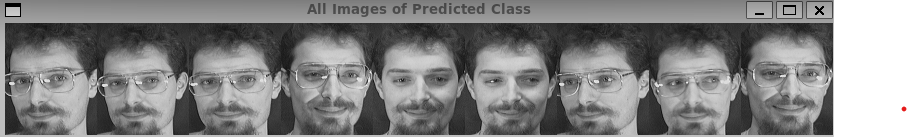
\includegraphics[scale = .85]{10fdb.png}    
\end{center}

\begin{lstlisting}[style=input]
 $$>$$ ./face_recognition attdatabase.txt 29
\end{lstlisting}

\begin{center}
    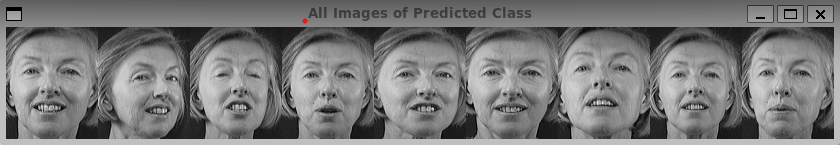
\includegraphics[scale = .85]{29fdb.png}    
\end{center}

\begin{lstlisting}[style=input]
 $$>$$ ./face_recognition attdatabase.txt 31
\end{lstlisting}
\begin{center}
    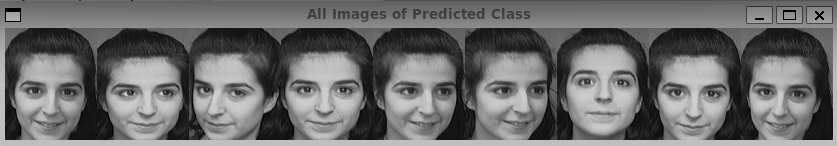
\includegraphics[scale = .85]{31fdb.png}    
\end{center}

\begin{lstlisting}[style=input]
 $$>$$ ./face_recognition attdatabase.txt 37
\end{lstlisting}

\begin{center}
    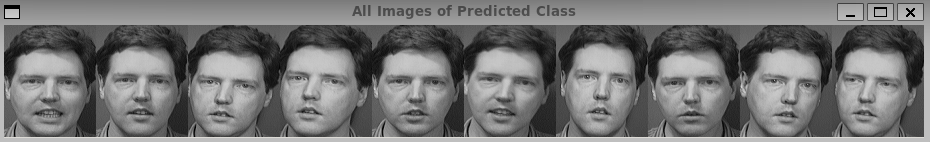
\includegraphics[scale = .77]{37fdb.png}    
\end{center}
\subsubsection{Facial Recognition Code}
\begin{lstlisting}[language=C++, caption=C++ code example]
/*
 * Copyright (c) 2011. Philipp Wagner <bytefish[at]gmx[dot]de>.
 * Released to public domain under terms of the BSD Simplified license.
 *
 * Redistribution and use in source and binary forms, with or without
 * modification, are permitted provided that the following conditions are met:
 *   * Redistributions of source code must retain the above copyright
 *     notice, this list of conditions and the following disclaimer.
 *   * Redistributions in binary form must reproduce the above copyright
 *     notice, this list of conditions and the following disclaimer in the
 *     documentation and/or other materials provided with the distribution.
 *   * Neither the name of the organization nor the names of its contributors
 *     may be used to endorse or promote products derived from this software
 *     without specific prior written permission.
 *
 *   See <http://www.opensource.org/licenses/bsd-license>
 */
#include "opencv2/core.hpp"
#include "opencv2/face.hpp"
#include "opencv2/highgui.hpp"
#include "opencv2/imgproc.hpp"
#include <iostream>
#include <fstream>
#include <sstream>
using namespace cv;
using namespace cv::face;
using namespace std;
static Mat norm_0_255(InputArray _src) {
    Mat src = _src.getMat();
    // Create and return normalized image:
    Mat dst;
    switch(src.channels()) {
    case 1:
        cv::normalize(_src, dst, 0, 255, NORM_MINMAX, CV_8UC1);
        break;
    case 3:
        cv::normalize(_src, dst, 0, 255, NORM_MINMAX, CV_8UC3);
        break;
    default:
        src.copyTo(dst);
        break;
    }
    return dst;
}
static void read_csv(const string& filename, vector<Mat>& images, vector<int>& labels, char separator = ';') {
    std::ifstream file(filename.c_str(), ifstream::in);
    if (!file) {
        string error_message = "No valid input file was given, please check the given filename.";
        CV_Error(Error::StsBadArg, error_message);
    }
    string line, path, classlabel;
    while (getline(file, line)) {
        stringstream liness(line);
        getline(liness, path, separator);
        getline(liness, classlabel);
        if(!path.empty() && !classlabel.empty()) {
            images.push_back(imread(path, 0));
            labels.push_back(atoi(classlabel.c_str()));
        }
    }
}
Mat concat_horizontally(const vector<Mat>& images) {
    if (images.empty()) {
        return Mat();
    }

    int max_height = 0;
    int total_width = 0;
    for (const Mat& image : images) {
        max_height = max(max_height, image.rows);
        total_width += image.cols;
    }

    Mat concatenated_image(max_height, total_width, images[0].type());
    int current_x = 0;
    for (const Mat& image : images) {
        Mat roi(concatenated_image, Rect(current_x, 0, image.cols, image.rows));
        image.copyTo(roi);
        current_x += image.cols;
    }

    return concatenated_image;
}
int main(int argc, const char *argv[]) {
    // Check for valid command line arguments, print usage
    // if no arguments were given.
    if (argc < 2) {
        cout << "usage: " << argv[0] << " <csv.ext> <output_folder> " << endl;
        exit(1);
    }
    string output_folder = ".";
    if (argc == 3) {
        output_folder = string(argv[2]);
    }
    // Get the path to your CSV.
    string fn_csv = string(argv[1]);
    size_t image_number = static_cast<size_t>(atoi(argv[2]));
    // These vectors hold the images and corresponding labels.
    vector<Mat> images;
    vector<int> labels;
    // Read in the data. This can fail if no valid
    // input filename is given.
    try {
        read_csv(fn_csv, images, labels);
    } catch (const cv::Exception& e) {
        cerr << "Error opening file \"" << fn_csv << "\". Reason: " << e.msg << endl;
        // nothing more we can do
        exit(1);
    }
    // Quit if there are not enough images for this demo.
    if(images.size() <= 1) {
        string error_message = "This demo needs at least 2 images to work. Please add more images to your data set!";
        CV_Error(Error::StsError, error_message);
    }
    // Get the height from the first image. We'll need this
    // later in code to reshape the images to their original
    // size:
    int height = images[0].rows;
    // The following lines simply get the last images from
    // your dataset and remove it from the vector. This is
    // done, so that the training data (which we learn the
    // cv::BasicFaceRecognizer on) and the test data we test
    // the model with, do not overlap.
    if (image_number >= images.size()) {
        cerr << "Invalid image number. Please provide a number between 0 and " << images.size() - 1 << "." << endl;
        exit(1);
    }
    Mat testSample = images[image_number];
    int testLabel = labels[image_number];
    images.erase(images.begin() + image_number);
    labels.erase(labels.begin() + image_number);

    // The following lines create an Eigenfaces model for
    // face recognition and train it with the images and
    // labels read from the given CSV file.
    // This here is a full PCA, if you just want to keep
    // 10 principal components (read Eigenfaces), then call
    // the factory method like this:
    //
    //      EigenFaceRecognizer::create(10);
    //
    // If you want to create a FaceRecognizer with a
    // confidence threshold (e.g. 123.0), call it with:
    //
    //      EigenFaceRecognizer::create(10, 123.0);
    //
    // If you want to use _all_ Eigenfaces and have a threshold,
    // then call the method like this:
    //
    //      EigenFaceRecognizer::create(0, 123.0);
    //
    Ptr<EigenFaceRecognizer> model = EigenFaceRecognizer::create();
    model->train(images, labels);
    // The following line predicts the label of a given
    // test image:
    int predictedLabel = model->predict(testSample);
    //
    // To get the confidence of a prediction call the model with:
    //
    //      int predictedLabel = -1;
    //      double confidence = 0.0;
    //      model->predict(testSample, predictedLabel, confidence);
    //
    string result_message = format("Predicted class = %d / Actual class = %d.", predictedLabel, testLabel);
    cout << result_message << endl;
    // Display all images of the person with the predicted class
    // Collect all images of the person with the predicted class
    vector<Mat> predicted_class_images;
    for (size_t i = 0; i < images.size(); ++i) {
        if (labels[i] == predictedLabel) {
            predicted_class_images.push_back(images[i]);
        }
    }

    // Concatenate images horizontally and display
    Mat concatenated_image = concat_horizontally(predicted_class_images);
    if (!concatenated_image.empty()) {
        imshow("All Images of Predicted Class", concatenated_image);
        waitKey(0);
    }

    // Here is how to get the eigenvalues of this Eigenfaces model:
    Mat eigenvalues = model->getEigenValues();
    // And we can do the same to display the Eigenvectors (read Eigenfaces):
    Mat W = model->getEigenVectors();
    // Get the sample mean from the training data
    Mat mean = model->getMean();
    // Display or save:
    if(argc == 2) {
        imshow("mean", norm_0_255(mean.reshape(1, images[0].rows)));
    } else {
        imwrite(format("%s/mean.png", output_folder.c_str()), norm_0_255(mean.reshape(1, images[0].rows)));
    }
    // Display or save the Eigenfaces:
    for (int i = 0; i < min(10, W.cols); i++) {
        string msg = format("Eigenvalue #%d = %.5f", i, eigenvalues.at<double>(i));
        cout << msg << endl;
        // get eigenvector #i
        Mat ev = W.col(i).clone();
        // Reshape to original size & normalize to [0...255] for imshow.
        Mat grayscale = norm_0_255(ev.reshape(1, height));
        // Show the image & apply a Jet colormap for better sensing.
        Mat cgrayscale;
        applyColorMap(grayscale, cgrayscale, COLORMAP_JET);
        // Display or save:
        if(argc == 2) {
            imshow(format("eigenface_%d", i), cgrayscale);
        } else {
            imwrite(format("%s/eigenface_%d.png", output_folder.c_str(), i), norm_0_255(cgrayscale));
        }
    }
    // Display or save the image reconstruction at some predefined steps:
    for(int num_components = min(W.cols, 10); num_components < min(W.cols, 300); num_components+=15) {
        // slice the eigenvectors from the model
        Mat evs = Mat(W, Range::all(), Range(0, num_components));
        Mat projection = LDA::subspaceProject(evs, mean, images[0].reshape(1,1));
        Mat reconstruction = LDA::subspaceReconstruct(evs, mean, projection);
        // Normalize the result:
        reconstruction = norm_0_255(reconstruction.reshape(1, images[0].rows));
        // Display or save:
        if(argc == 2) {
            imshow(format("eigenface_reconstruction_%d", num_components), reconstruction);
        } else {
            imwrite(format("%s/eigenface_reconstruction_%d.png", output_folder.c_str(), num_components), reconstruction);
        }
    }
    // Display if we are not writing to an output folder:
    if(argc == 2) {
        waitKey(0);
    }
    return 0;
}

\end{lstlisting}\\
\begin{center}
    \tiny https://docs.opencv.org/4.x/da/d60/tutorial\_face\_main.html
\end{center}
\newpage
\section{Conclusion}
In this report, we have covered the main aspects of Singular Value Decomposition (SVD) and how it is used in various industries that utilize machine learning. Through reviewing important linear algebra concepts used in computing SVD and SVD-based algorithms, we have seen that the systems that utilize SVD can efficiently and quickly process data in image compression, facial recognition, and recommender systems.

The SVD++ algorithm developed for Netflix is an excellent example of how powerful and efficient SVD can be when processing large amounts of data and extracting useful information required to carry out machine learning tasks. As technology and artificial intelligence continue to advance, and their usage grows, SVD-based algorithms are increasingly useful tools that we should continue to explore.

In conclusion, we can say that Singular Value Decomposition is an important mathematical concept that plays a significant role in the field of machine learning. It has become an essential tool for data scientists, engineers, and researchers who work on problems that involve the analysis and processing of large amounts of data. By understanding the underlying principles of SVD and its applications, we can build more efficient and accurate machine learning models that can help us solve complex problems in various domains.
\newpage
\section{References}
\begin{thebibliography}{9}

\bibitem{shen2019linear}
Shen, L., Wang, H., \& Wojdylo, J. (2019). Linear Algebra. Springer International Publishing, pp. 130-139.

\bibitem{chen2005symmetrical}
Chen, Y., Tong, S., Cong, F., \& Xu, J. (2005). Symmetrical singular value decomposition representation for pattern recognition.

\bibitem{analyticsindiamag}
Analytics India Magazine. (n.d.). Singular Value Decomposition (SVD) - Application in Recommender Systems. Retrieved from \url{https://analyticsindiamag.com/singular-value-decomposition-svd-application-recommender-system/}

\bibitem{stewart1993early}
Stewart, G. W. (1993). On the early history of Singular Value Decomposition. SIAM Review, 35(4), 551-556.

\bibitem{eigenvectors}
Margalit, D., \& Rabinoff, J. (n.d.). Eigenvalues and Eigenvectors. Interactive Linear Algebra textbook by Dan Margalit and Joseph Rabinoff. Retrieved from \url{https://textbooks.math.gatech.edu/ila/eigenvectors.html}

\bibitem{boia2011image}
Boia, R. T., Verli, F., Netto, M. L. C., de Faria, A. E., \& de Albuquerque, V. H. C. (2011). Image-based PCA and SVM algorithm for automatic detection of oil spillages in the ocean. MDPI Sensors, 11(7), 369-381.

\bibitem{brems2017one}
Brems, M. (2017, April 17). A One-Stop Shop for Principal Component Analysis. Towards Data Science. Retrieved from \url{https://towardsdatascience.com/a-one-stop-shop-for-principal-component-analysis-5582fb7e0a9c}

\bibitem{dynamsoft2019color}
Dynamsoft. (2019, May 24). Image Processing 101 Chapter 1.3: Color Space Conversion. Retrieved from \url{https://www.dynamsoft.com/blog/insights/image-processing/image-processing-101-color-space-conversion/}

\bibitem{researchgate}
Mackey, L., \& Gwayi, D. (2016). Principal Component Analysis - A Tutorial. ResearchGate. Retrieved from \url{https://www.researchgate.net/publication/309165405_Principal_component_analysis_-_a_tutorial}

\bibitem{cuemath}
Cuemath. (n.d.). Covariance Matrix. Retrieved from \url{https://www.cuemath.com/algebra/covariance-matrix/}

\bibitem{facerecognition}
Brownlee, J. (2019). Face Recognition using Principal Component Analysis. Machine Learning Mastery. Retrieved from \url{https://machinelearningmastery.com/face-recognition-using-principal-component-analysis/}

\bibitem{dynamsoft2019facerecognition}
Dynamsoft. (n.d.). Image Processing 101: Color Space Conversion. Retrieved from \url{https://www.dynamsoft.com/blog/insights/image-processing/image-processing-101-color-space-conversion/}

\bibitem{laid}
Delanover. (n.d.). Explanation: Face Recognition using Eigenfaces. Retrieved from \url{https://laid.delanover.com/explanation-face-recognition-using-eigenfaces/}
\end{thebibliography}

\end{document}